%!TEX root = main.tex
In this section, we evaluate the performance of the proposed MARL-based resource allocation approach on several instances containing IAB-nodes working in FD or HD mode, mobile UEs, and random link failures caused by mobile obstacles. Every value shown in the figures of this section is the result of an average over 10 random instances.

\vspace{-11pt}
\subsection{Scenario Settings}
In line with 3GPP NR IAB simulation guidelines \cite{3gpp15study}, we consider a $300$m$\times300$m service area where 1 IAB-donor is located at the left-side midpoint and 4 IAB-nodes are randomly deployed in the area. Fig.~\ref{fig:example_simulation_scenarios} shows two examples of backhaul deployment of IAB network scenarios.
A set of 30 UEs move around in the area, with random initial positions and directions. The considered heights of the IAB-donor, IAB-nodes and UEs are $25$m, $6$m and $1.5$m, respectively.
Both the IAB-donor and IAB-nodes are equipped with $N_p=4$ antenna panels, each of which contains $8\times6$ elements and manages $N_s=5$ sectors.
The transmission power of each panel at the IAB-donor and IAB-nodes is respectively $29.3$ dBm and $20.3$ dBm. The receiver noises at the IAB-nodes and UEs are $-84.023$ dBm and $-82.023$ dBm, respectively. The azimuth HPBWs for the IAB-donor and IAB-nodes are $\pi/36$ and $\pi/12$, and the elevation HPBW is $\pi/4$ for both. The SINR thresholds and rates considered for the access and backhaul links are those indicated in MCS Index Table 3 for PDSCH in the 3GPP NR specification \cite{3gpp17PhysicalData}. Finally, one frame consists of $80$ slots, each with a duration of $\delta=125\mu$s, which correspond to the in-band IAB at $28$ GHz, $400$ MHz bandwidth, NR Numerology \#$3$ ($120$ kHz subcarrier spacing).

\textbf{User mobility:}
UEs move in the playground according to a Random Waypoint model \cite{bai2004survey}. Specifically, a UE randomly selects a direction in the angular range $\xi \in [-180^\circ, 180^\circ]$ from the current direction. Then it travels along the selected direction with a constant speed uniformly chosen within the range $[2, 20]$m/s (or $[20,60]$m/s in the extended analysis). Speeds and directions of different UEs are selected independently and randomly. After moving for $t_{m}\in [2, 6]$s, a UE pauses for an interval $t_{p}\in [0, 1]$s before resuming. UEs bounce back when they reach the area boundary.

\textbf{Obstacles:}
We assess the performance of our approach according to two levels of obstacle densities in the area and refer to them as \emph{low obstacle density (LOD)} and \emph{high obstacle density (HOD)}. They are implemented by dropping in the simulated service area, respectively, $15$ and $60$ cylindrical obstacles with a radius of $2.5$m and a height of $2$m. They move at a speed of $2$m/s - $20$m/s following the same Random Waypoint model applied to UEs.

\begin{figure}
    \centering
    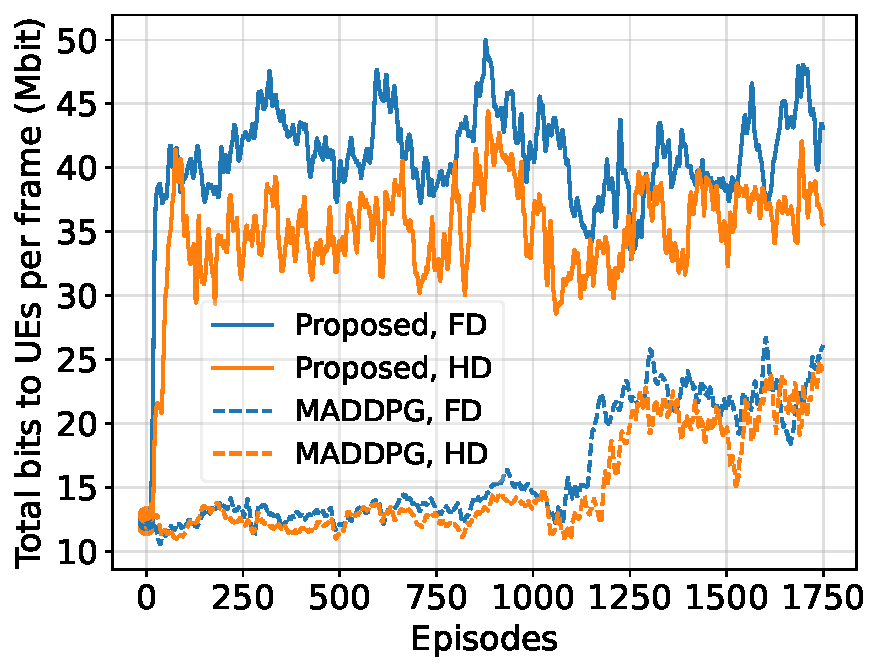
\includegraphics[width=0.8\linewidth]{figures/TON_revision/training_curve_bits_fd_hd_more.pdf}
    \caption{\small Training curves for FD and HD IAB networks (with user speeds in the range of 2-20m/s and under HOD condition).}
    \label{fig:training_curves_fd_hd}
    \vspace{-2mm}
\end{figure}

\begin{figure}[!t]
    \centering
    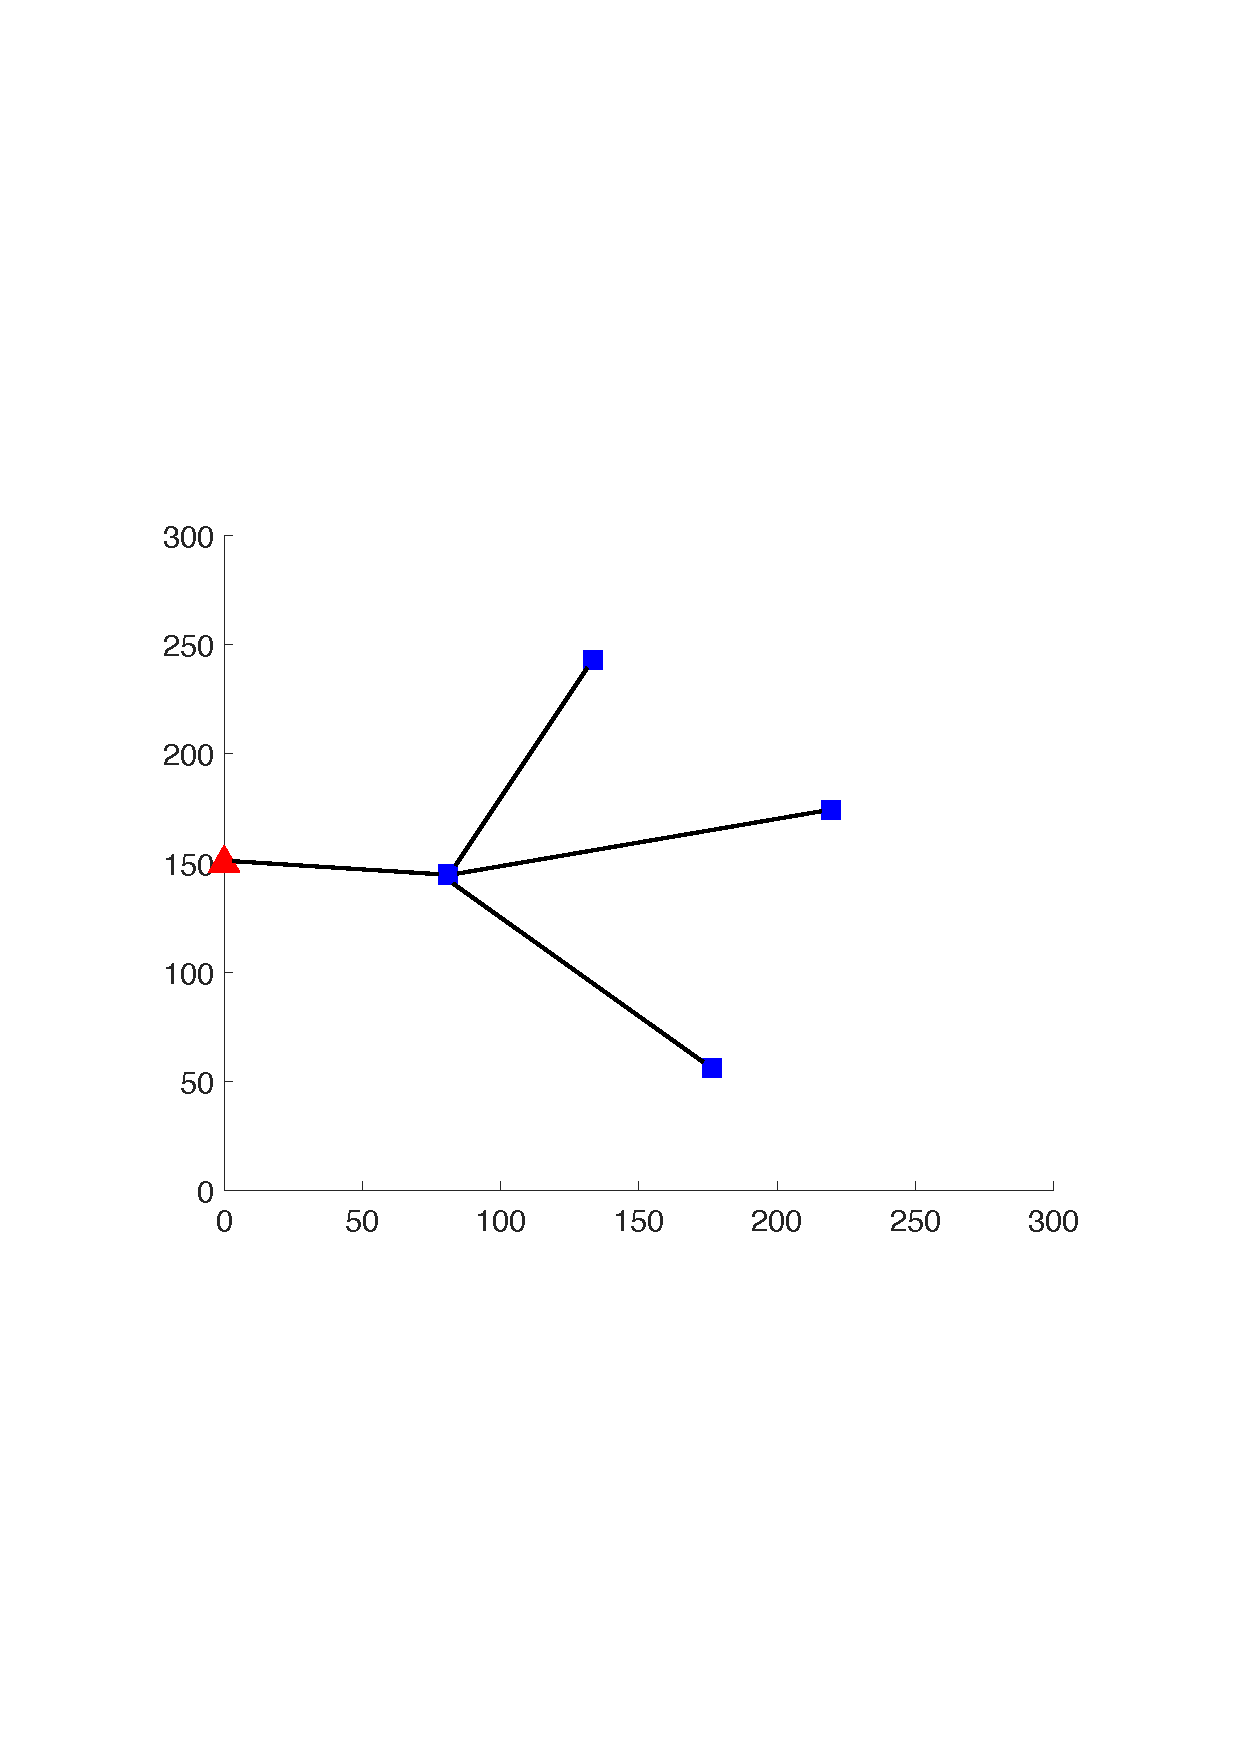
\includegraphics[width=0.48\linewidth]{figures/TON_revision/scenario1_exp.pdf}
    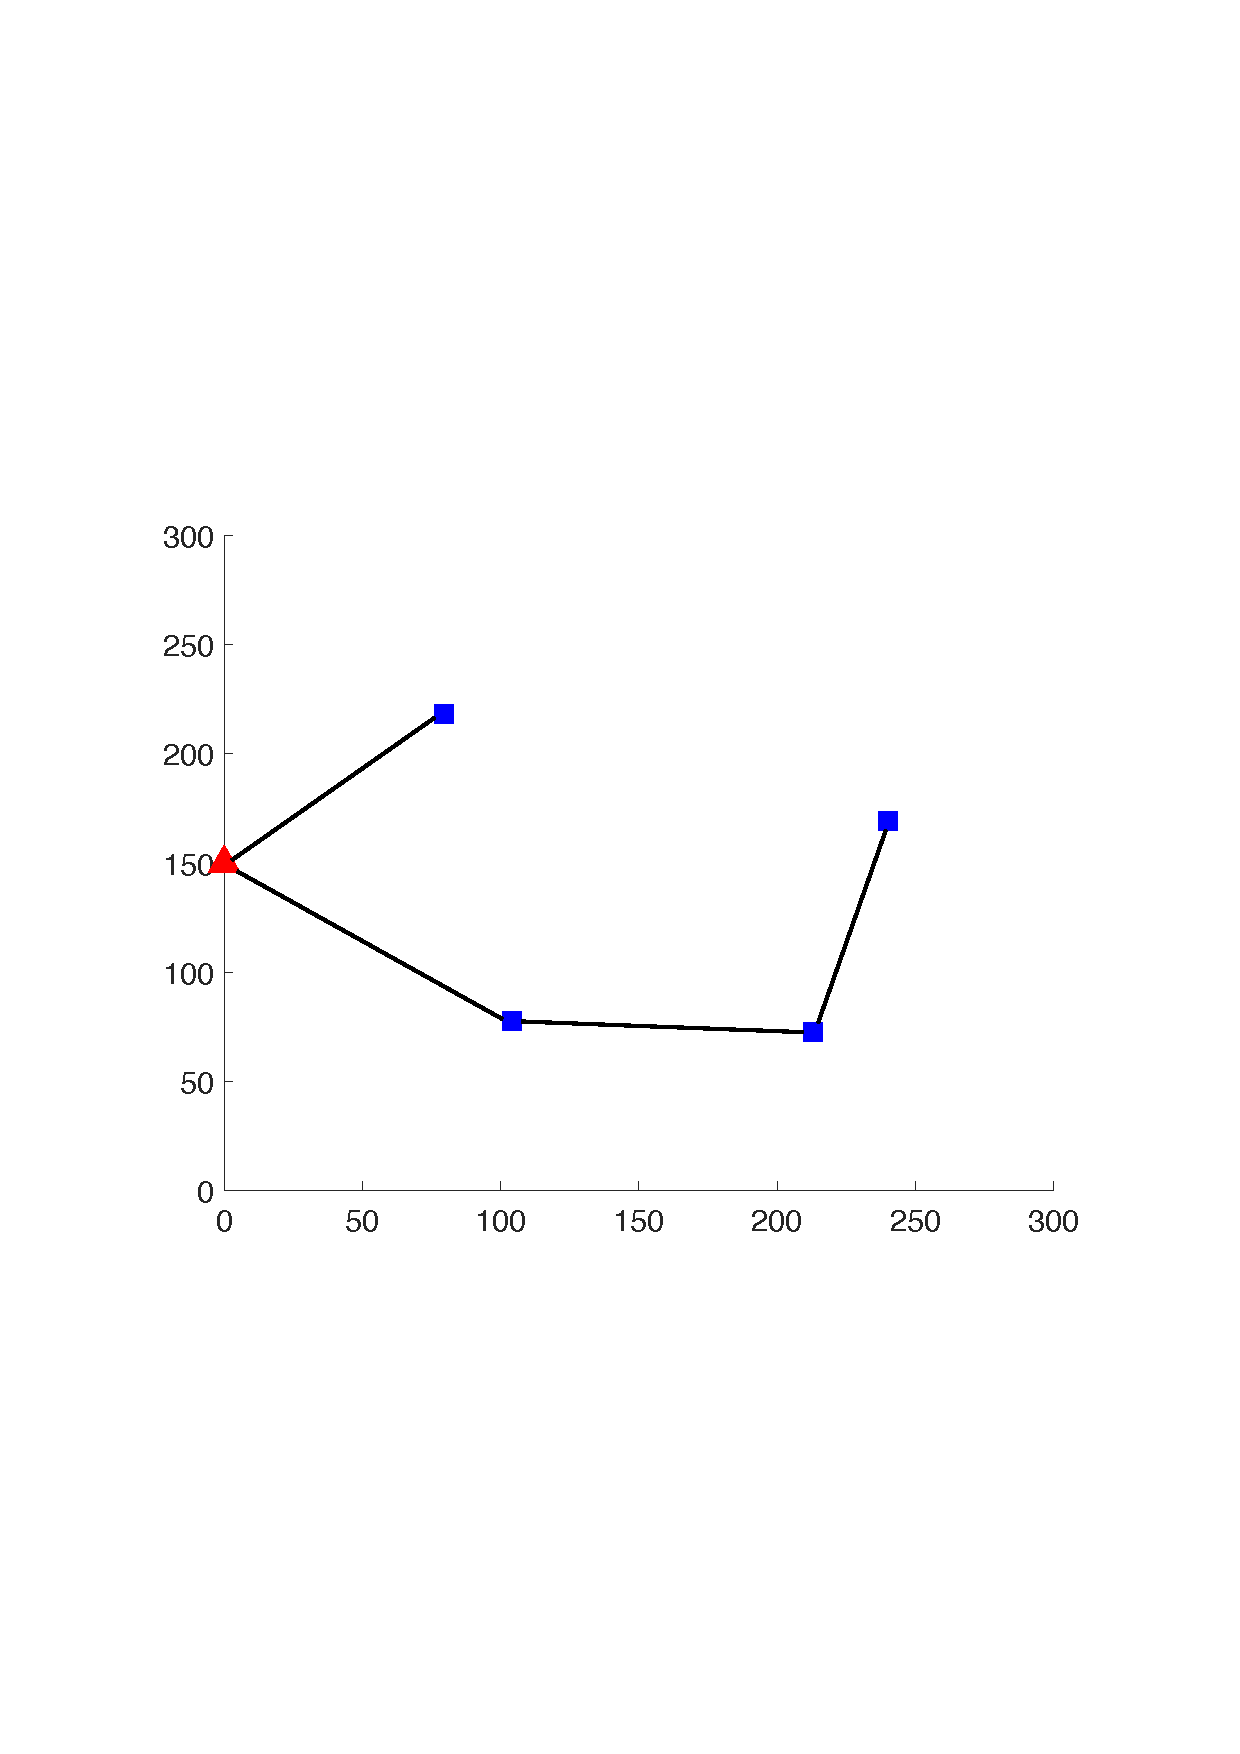
\includegraphics[width=0.48\linewidth]{figures/TON_revision/scenario2_exp.pdf}
    \caption{Example IAB network scenarios considered in the experiments (red triangle: IAB-donor, blue squares: IAB-nodes, black lines: backhaul links).}
    \label{fig:example_simulation_scenarios}
\end{figure}

\vspace{-12pt}
\subsection{MARL Model Settings}
We train each DNN model of our approach based on the experience data of $5000$ episodes, each of which consists of $T=80$ steps (slots).
This corresponds to a training period of $5000$ frames, thus a total time of $50$s. All the DNN models have a hidden dimension of $128$. We consider $K=4$ consecutive DNN updates, a data collection period of $T_{upd}=100$ steps, and a warm-up period of $T_{wup}=10$ episodes. The updates are performed via Adam optimizer with a learning rate of $0.001$ for both distributed policies and centralized critics. The weight $\rho_{BH}$ for backhaul transmission in the reward function is empirically set to $0.8$. The discount factor $\gamma $ is $0.99$ and the weight $\tau$ of the policy entropy is set to $0.01$. The weight vector $\bar{\psi}$ of the target critic network, similarly to $\bar{\theta}$ of the target actor network, is updated via $\bar{\psi} = \kappa\bar{\psi} + (1-\kappa)\psi$ with update rate $\kappa = 0.001$. The replay buffer $H$ has a maximum length of $10^6$ entries, and each update uses a mini-batch of $1024$ entries, randomly sampled from $H$.

The settings of the DNN architectures and training hyper-parameters for MADDPG baseline approach are the same accordingly.  


Training curves expressing the total traffic volume delivered in a frame from the IAB-donor to all the UEs (which corresponds to the throughput objective of the resource optimization problem) are shown in Fig. \ref{fig:training_curves_fd_hd}, where IAB-nodes operate in FD and HD modes, respectively. To better appreciate the learning trend, we only show the first $1750$ episodes, which involve the key performance-improving period.
As we can see, compared with the MADDPG approach that shows apparent throughput boost after $1000$ episodes, the training process of the proposed approach shows an immediate throughput increase in both FD and HD cases. Indeed, blue and orange curves can reach high values within $100$ episodes, showing the models can learn fast from the experience. Nevertheless, we train both approaches up to $5000$ episodes to let them accumulate sufficient experience and eventually obtain a stable performance in any situation. Moreover, the proposed approach can achieve almost double throughput of the MADDPG, which is consistent with
Figs.~\ref{fig:bars_fd}, \ref{fig:bars_hd}, \ref{fig:cdf_datarate}.

\vspace{-10pt}
\subsection{Performance Analysis}

\begin{figure*}
\centering
    \begin{subfigure}[b]{0.32\textwidth}
            \centering
            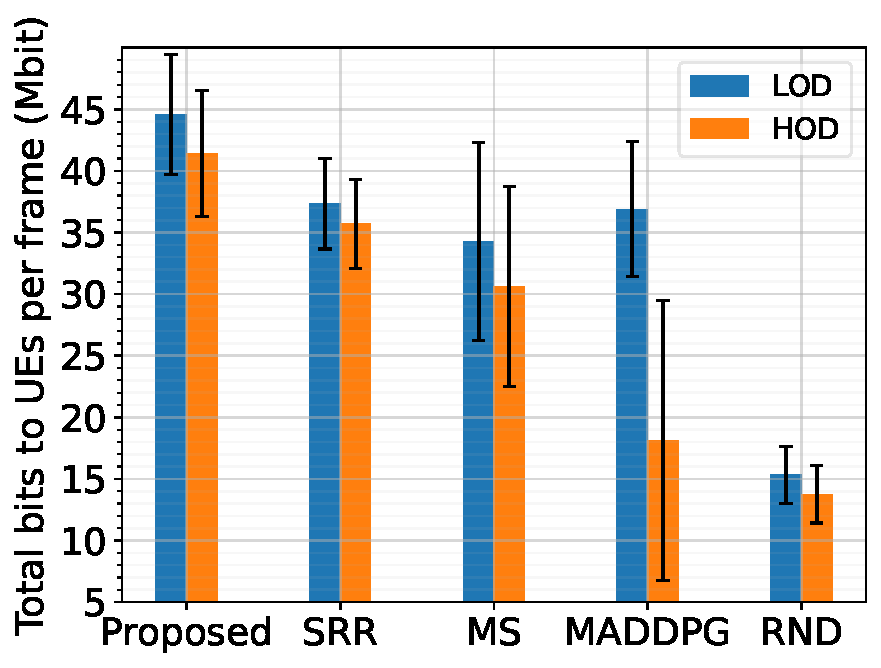
\includegraphics[width=\linewidth]{figures/TON_revision/total_bits_fd.pdf}
            \caption{\small Avg. bit volume delivered per frame.}
            \label{total_bits_fd}
    \end{subfigure}
    \begin{subfigure}[b]{0.32\textwidth}
            \centering
            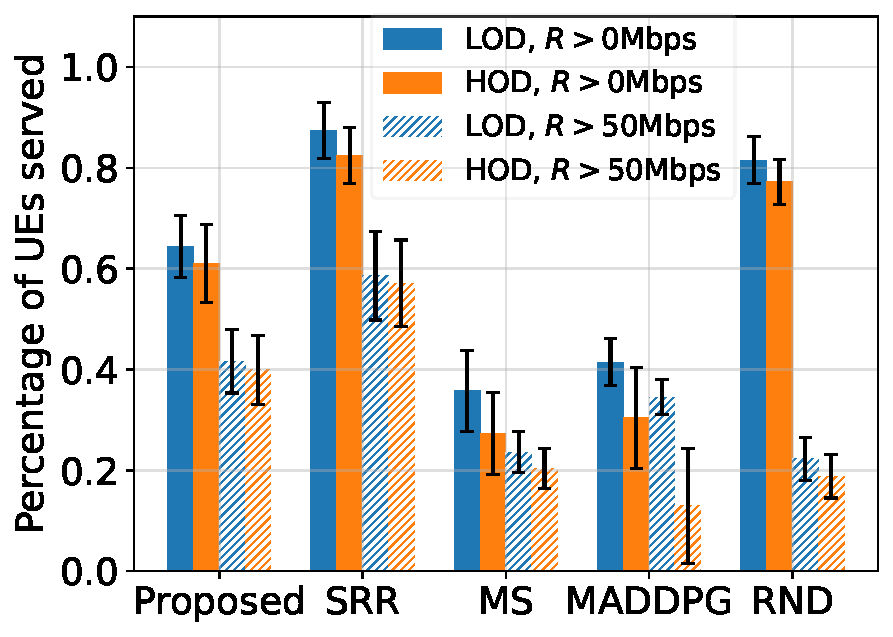
\includegraphics[width=\linewidth]{figures/TON_revision/served_percent_fd.pdf}
            \caption{\small Avg. percent of served UEs per frame.}
            \label{UE_percent_fd}
    \end{subfigure}
    \begin{subfigure}[b]{0.32\textwidth}
            \centering
            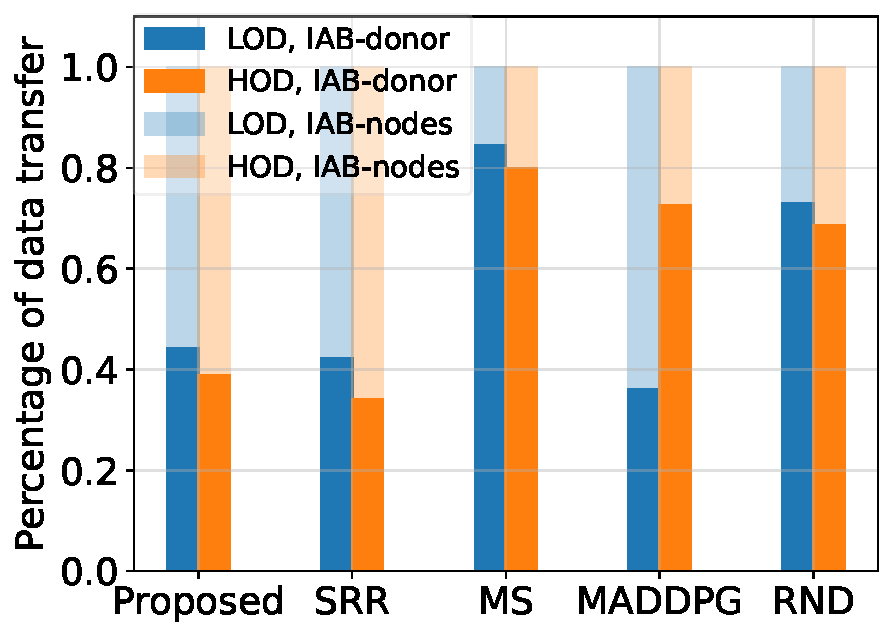
\includegraphics[width=\linewidth]{figures/TON_revision/BSRN_percent_fd.pdf}
            \caption{\small Avg. traffic volume split per frame.}
            \label{BSRN_percent_fd}
    \end{subfigure}
    \caption{\small Performance comparison of the five schemes in FD IAB networks.}
    \label{fig:bars_fd}
    \vspace{-4mm}
\end{figure*}

\begin{figure*}
\centering
    \begin{subfigure}[b]{0.32\textwidth}
            \centering
            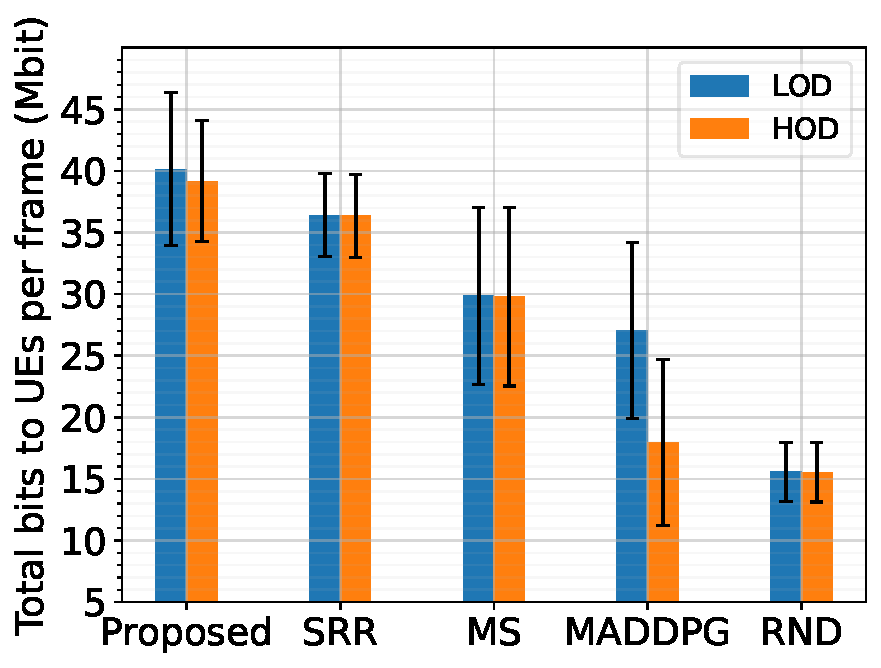
\includegraphics[width=\linewidth]{figures/TON_revision/total_bits_hd.pdf}
            \caption{\small Avg. bit volume delivered per frame.}
            \label{total_bits_hd}
    \end{subfigure}
    \begin{subfigure}[b]{0.32\textwidth}
            \centering
            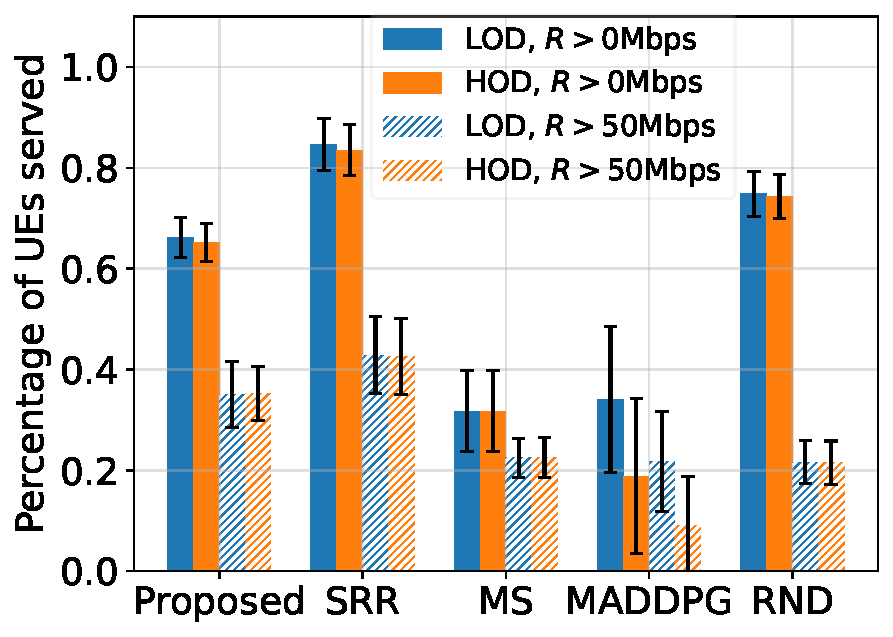
\includegraphics[width=\linewidth]{figures/TON_revision/served_percent_hd.pdf}
            \caption{\small Avg. percent of served UEs per frame.}
            \label{UE_percent_hd}
    \end{subfigure}
    \begin{subfigure}[b]{0.32\textwidth}
            \centering
            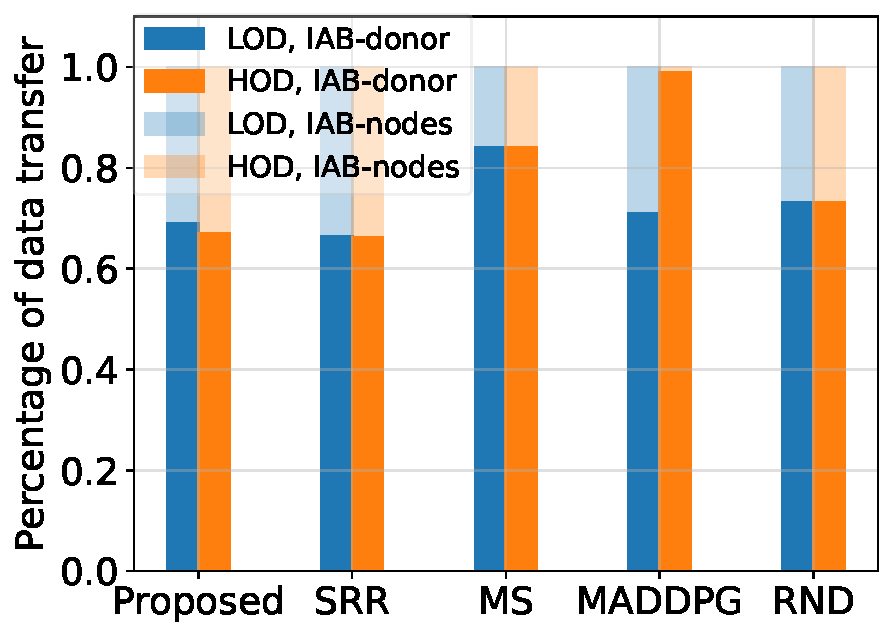
\includegraphics[width=\linewidth]{figures/TON_revision/BSRN_percent_hd.pdf}
            \caption{\small Avg. traffic volume split per frame.}
            \label{BSRN_percent_hd}
    \end{subfigure}
    \caption{\small Performance comparison of the five schemes in HD IAB networks.}
    \label{fig:bars_hd}
    \vspace{-4mm}
\end{figure*}

\begin{figure*}
\centering
    \begin{subfigure}[b]{0.38\textwidth}
		\centering
   		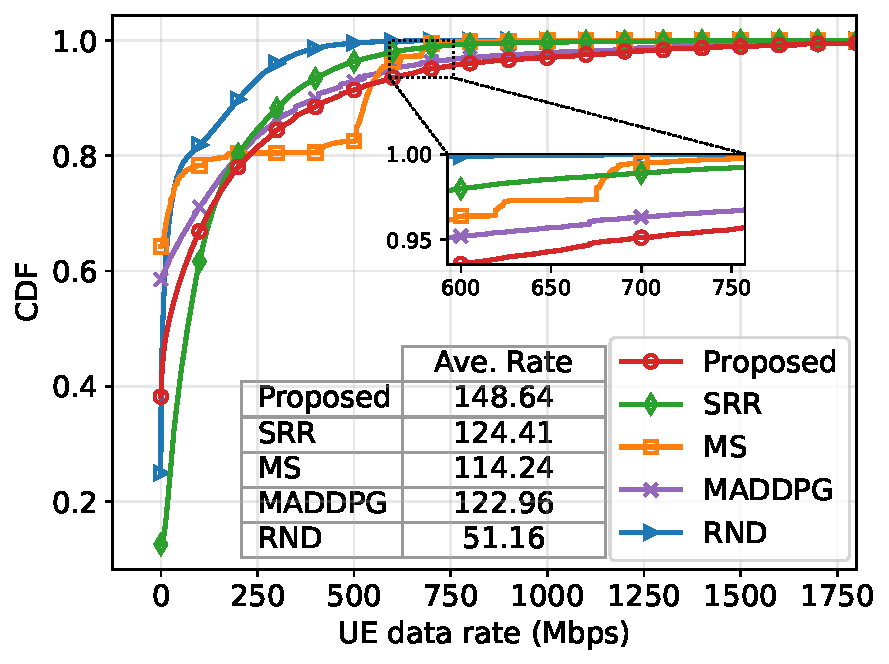
\includegraphics[width=\linewidth]{figures/TON_revision/CDF_ue_rate_fd.pdf}
		\caption{\small UE data rate in the FD case.}
    	\label{fig:cdf_fd}
	\end{subfigure}
	\begin{subfigure}[b]{0.38\textwidth}
   		\centering
  		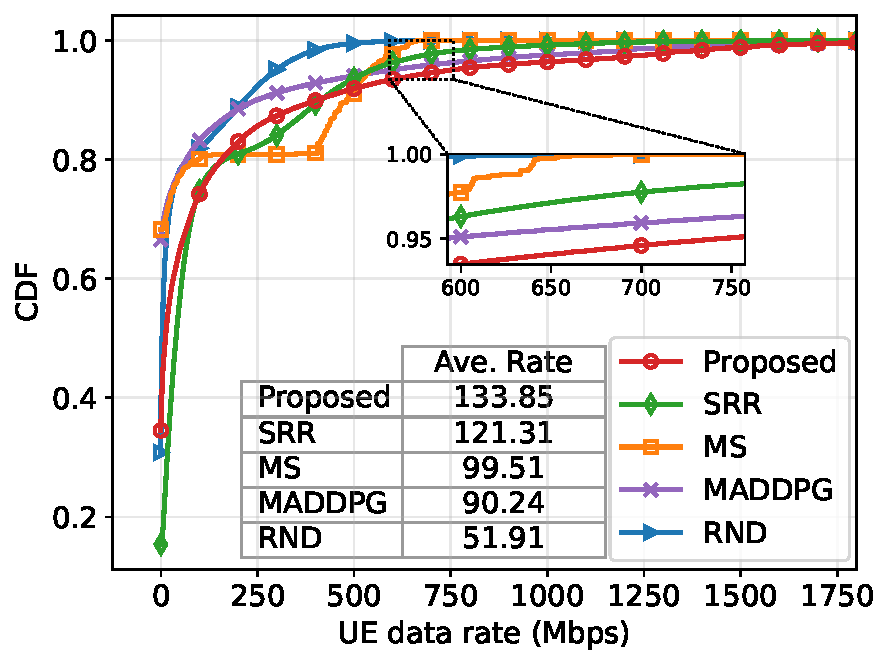
\includegraphics[width=\linewidth]{figures/TON_revision/CDF_ue_rate_hd.pdf}
   		\caption{\small UE data rate in the HD case. }
  		\label{fig:cdf_hd}
	\end{subfigure}
	\caption{\small CDF of the data rate achieved by each UE in a frame, under the LOD condition.}
	\label{fig:cdf_datarate}
        \vspace{-5mm}
\end{figure*}

\begin{figure*}
\centering
    \begin{subfigure}[b]{0.38\textwidth}
   		\centering
  		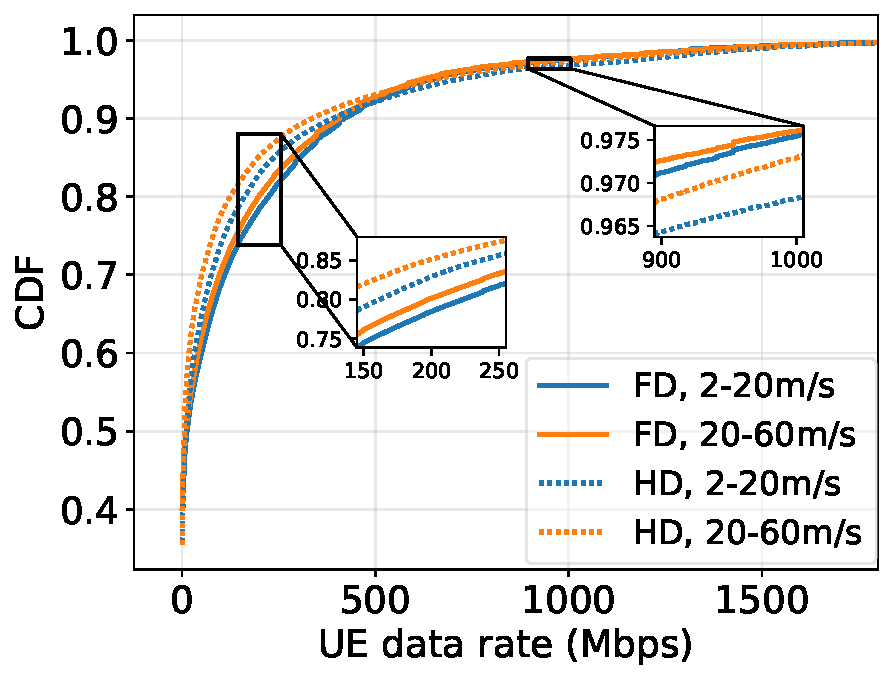
\includegraphics[width=\linewidth]{figures/revision/highspeed_UERateCDF_noaverage.pdf}
   		\caption{\small CDF of UE data rate.}
  		\label{fig:diff_speed_count_for_every_ue}
	\end{subfigure}
    \begin{subfigure}[b]{0.38\textwidth}
		\centering
   		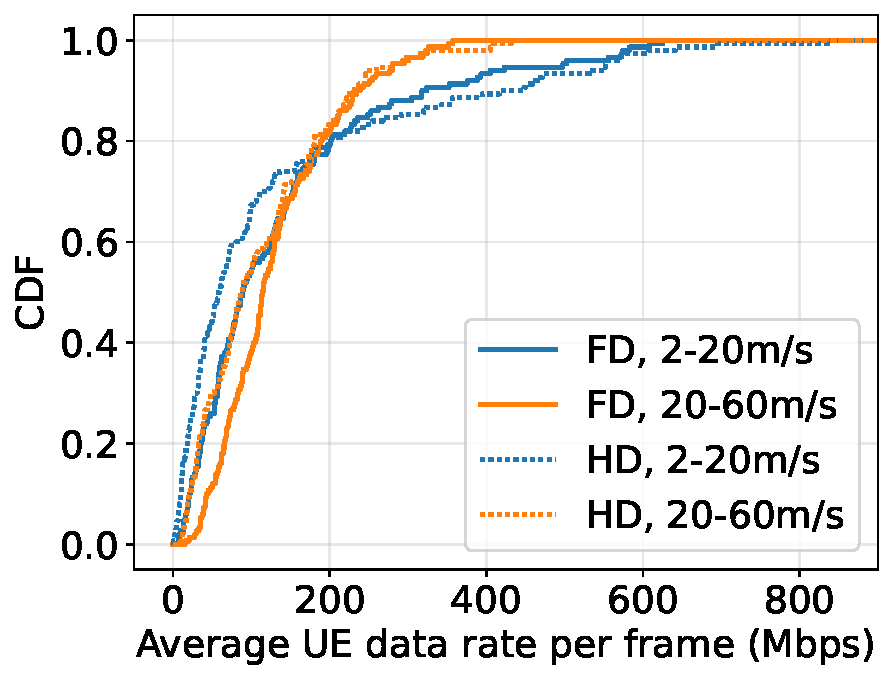
\includegraphics[width=\linewidth]{figures/revision/highspeed_UERateCDF_average.pdf}
		\caption{\small CDF of average UE data rate per frame.}
    	\label{fig:diff_speed_average_per_frame}
    \end{subfigure}
	\caption{\small CDFs of the UE data rates achieved at different UE speeds and duplex modes.}
	\label{fig:cdf_diff_speed}
    \vspace{-6mm}
\end{figure*}

We compare the proposed MARL-based approach (referred to as \textit{Proposed} in the following) against four representative schemes:
\begin{itemize}
	\item Super Round-Robin scheme (referred to as \textit{SRR}):\\
    A common scheduling scheme when dealing with wireless access transmissions, where each panel of the IAB-donor and IAB-nodes iteratively serves slot-by-slot every UE under its coverage in round-robin fashion. In this scheme, all the IAB-nodes are assumed to always have data bits to deliver, which is guaranteed by the automatic IAB-node's buffer refill from its parent node when its number of bits drops below a certain threshold. This is an ideal behavior (the reason why it is named ``super"); indeed, a proper refilling strategy must be designed. \textit{SRR}'s performance provides an upper bound on the performance of any real round-robin implementation.
	\item Multi-Slot algorithm (referred to as \textit{MS}):\\
 A heuristic algorithm proposed in \cite{saad2019millimeter} to perform link scheduling. This algorithm generates a sequence of link sets, each of which contains a group of links that can be simultaneously activated in a slot satisfying the SINR conditions required by activated MCSs. Based on this algorithm, we periodically generate the compatible link sets (e.g., every frame) or timely regenerate the link sets every time the network layout undergoes a change due to mobile users, and iteratively apply them in a sequential order, slot by slot, till the next link set generation.
        
        \item MADDPG-based scheme (referred to as \textit{MADDPG}):\\ A scheme obtained through training the agents formulated in Sec~\ref{method} based on MADDPG algorithm \cite{maddpg}. 
        
        \item Random scheme (referred to as \textit{RND}):\\
        A random scheduling scheme where each panel randomly picks an action from its candidate action set.
\end{itemize}

We begin the analysis for both FD and HD cases by considering typical UE urban speeds, in the range of $2$m/s - $20$m/s, to assess the impact of different obstacle densities on the performance. Results are shown in Figs. \ref{fig:bars_fd}-\ref{fig:cdf_datarate}. Then, we extend our analysis to consider different speed ranges, as reported in Fig. \ref{fig:cdf_diff_speed}. We refer readers to Appendix Sec. B for a complexity and scalability analysis of the system.

\textbf{Traffic Volume:}
Figs. \ref{total_bits_fd} and \ref{total_bits_hd} show the average overall traffic volume delivered to UEs per frame, respectively in the FD case and in the HD case, considering both the LOD and HOD blockage situations.

Compared to \textit{SRR}, which assumes an ideal refilling strategy for IAB-nodes' buffers, the \textit{Proposed} can achieve an improvement of $20\%$ in the FD case and $10\%$ in the HD case. This is because the \textit{Proposed} can coordinate the interference among links and adapt its decisions to UE mobility and obstacle obstructions. The reduced gain in the HD mode is mainly due to the limited degrees of freedom caused by HD constraints at IAB-nodes.
Indeed, on one side, an IAB-node's buffer needs to be refilled through backhaul transmissions in order not to bottleneck downstream access transmissions, on the other, backhaul transmissions to the IAB-node preclude its access transmissions due to HD constraints.
In practice, these HD limitations prevent smart resource allocation schemes from fully exploiting all available wireless resources.
Nevertheless, in the HD case, the \textit{Proposed} approach can still achieve an advantage of almost $500$Mbps over \textit{SRR}.

Moreover, the \textit{Proposed} outperforms \textit{MS} by $30\%$ in FD case and $35\%$ in HD case. Although \textit{MS} provides a near-optimal interference coordination and its compatible link sets are ideally regenerated whenever it is needed, this cannot compensate the \textit{Proposed}'s advantages, which timely recharges IAB-nodes' buffers and on-the-fly adapts to obstacle blockages. In addition, we can observe an interesting aspect: \textit{SRR} performing better than \textit{MS} demonstrates how a good IAB-nodes' buffer management has a larger impact on the data transfer than link interference coordination.


Furthermore, despite sharing the same RL components, the \textit{Proposed} outperforms the \textit{MADDPG} by around $20\%$ and $60\%$ in LOD and HOD conditions for FD networks, and around $50\%$ and $55\%$ for HD networks, respectively. This primarily stems from the distinct model architectures, especially the attention-based central critics, and training procedures of the \textit{Proposed} and \textit{MADDPG}.



Finally, according to the error bars at the tips of grouped bars, which represent the standard deviations of the throughput delivered to UEs, \textit{RND} and \textit{SRR} exhibit the smallest variance, while the \textit{MS} and \textit{MADDPG} show the largest variance. The variance of the \textit{Proposed} approach is reasonably small, which demonstrates a stable performance across different network scenario instances.


\textbf{Coverage:}
Figs. \ref{UE_percent_fd} and \ref{UE_percent_hd} indicate the average percentage of UEs served per frame. We adopt two definitions of served UEs: in the first one, a UE is declared as served if it experiments a data rate in a frame larger than $0$Mbps ($R>0$Mbps in the figures), while the second definition introduces a minimum data rate threshold of $50$Mbps ($R>50$Mbps in figures). Similarly to the previous traffic volume figures, results in both the LOD and HOD conditions are shown.

Some evident aspects emerge from the figures. Considering the minimum data rate of $0$Mbps, both \textit{SRR} and \textit{RND} show higher percentages of $(R>0)$-served UEs than the \textit{Proposed} scheme. This is a consequence of the throughput-vs.-fairness trade-off. While \textit{SRR} and \textit{RND} reach all UEs with the same probability thus providing the best fairness, the \textit{Proposed} tends to preferably serve those UEs that can bring the best overall throughput. However, when considering UEs that are served with at least $50$Mbps, the gap between \textit{SRR} and the \textit{Proposed} remarkably reduces and the \textit{Proposed} even outperfoms \textit{RND}. This confirms that the service percentages guaranteed by \textit{SRR} and \textit{RND} are mainly driven by UEs with very-low data rates. This further demonstrates that the proposed resource allocation scheme can very effectively deal with such complex network scenarios.

\textbf{Backhaul Load:}
Figs. \ref{BSRN_percent_fd} and \ref{BSRN_percent_hd} provide an insight into the average fraction of the traffic delivered to UEs through the IAB wireless backhaul per frame. The upper translucent part of each bar represents the average percentage of the data volume received by UEs from IAB-nodes via multi-hops, while the lower opaque part reports the complementary percentage of the traffic directly received from the IAB-donor. We can see that the \textit{Proposed} aggressively resorts to backhaul IAB-nodes when operating in FD mode, even if the larger panels and the higher transmission power of the IAB-donor may lead UEs to directly connect to it. In the HD case, all the considered schemes reduce the load of the wireless backhaul. Indeed, HD IAB-nodes are less effective in relaying traffic flows, thus limiting wireless link transmission concurrency, especially in the IAB tree topology.

\textbf{CDF of Per-UE Data Rate:}
Figs. \ref{fig:cdf_fd} and \ref{fig:cdf_hd} compare the performance of the five schemes in terms of per-UE data rate cumulative distribution function (CDF). As the CDF curves show very similar trends under LOD and HOD conditions, we only show LOD curves. We measure the per-UE data rate frame by frame, whose values are used to compute the CDF.

As we can see from the upper right corner of the figures, the maximum rate achieved by the \textit{Proposed} is near 1800 Mbps in both FD and HD cases, which remarkably exceeds the other four schemes.
This means that the problem faced is not trivial and only a careful link scheduling scheme can allow a good performance. In addition, this further proves that the \textit{Proposed} can discover the most effective strategy to increase the overall throughput.

Moreover, it is evident that the order of the five schemes to serve high per-UE data rate is: the \textit{Proposed}, \textit{MADDPG}, \textit{SRR}, \textit{MS} and \textit{RND}. This shows an interesting point that in order to maximize total throughput, learning-based approaches (\textit{Proposed} and \textit{MADDPG}) tend to pursue large per-UE data rate rather than serve a large number of UEs with average per-UE data rate.


The CDF values on the leftmost side indicate the percentage of users that cannot be served. This information has been better described through the solid bars ($R>0$Mbps) in Figs. \ref{UE_percent_fd} and \ref{UE_percent_hd}, however, here we can see how \textit{SRR} and \textit{RND} schemes show the highest probabilities for small rate values, because they do not tend to select the best UEs to maximize the overall throughput, but rather to reach all UEs with the same probability, although with a small throughput.

\textbf{UE Speed Sensitivity:}
Fig. \ref{fig:cdf_diff_speed} shows the performance of the \textit{Proposed} scheme over different speed ranges in both FD and HD cases. As the plots for the LOD and HOD cases are very similar, we only show the one of the HOD case. In particular, we observe the per-UE data rate CDF from two perspectives.
On one hand, as shown in Fig. \ref{fig:diff_speed_count_for_every_ue}, we adopt the same approach as in Fig. \ref{fig:cdf_datarate}, where we collect UE data rates frame by frame and compute the CDF based on all the collected rate values.
On the other, as shown in Fig. \ref{fig:diff_speed_average_per_frame}, we average the data rate of each UE over all the frames and compute the CDF based on per-UE data rate averages.

Fig. \ref{fig:diff_speed_count_for_every_ue} shows us that despite different speed ranges, the CDF curves corresponding to the same duplex mode are close. This implies that although the UE speed evidently affects the average UE data rate as indicated by Fig. \ref{fig:diff_speed_average_per_frame}, it has in practice a negligible impact on the distribution of the per-frame data rate across different UEs.

From Fig. \ref{fig:diff_speed_average_per_frame}, we can see that in both the FD and HD cases, increasing UE speeds reduces average UE data rates. This is reasonable because extremely fast-moving UEs can lead to more frequent and impactful network status changes.
However, even at the extremely high speeds of $[20,60]$m/s, which can be rarely seen in the urban scenarios where such IAB networks are envisioned, the impact on the performance is limited.